% !TEX root=../../Thesis.tex
\newcommand {\matr}[2]{\left[\begin{array}{#1}#2\end{array}\right]}

\chapter{Modeling Intersection Driving Scenarios}
\label{ch:modeling_intersection}
% \begin{center}
%   \textit{\textbf{RQ 1: How can \gls{rl} be used to create a decision-making agent for driving through intersections?}}
% \end{center}
%   \vspace{12pt}

Navigating an intersection is a sequential decision-making problem that can be mathematically modeled using an \gls{mdp}, as introduced in Section~\ref{sec:background_mdp}. This thesis focuses on driving through intersections in the presence of other drivers, emphasizing not only to follow traffic rules but also the ability to adapt to the intentions of other drivers. Given that current sensors cannot directly observe other drivers' intentions, a \gls{pomdp} is a more suitable framework for formulating this problem.

This chapter explores the modeling of intersection driving scenarios for autonomous vehicles. 

\section{POMDP formulation}
\label{sec:pomdp_fomulation}
Effectively modeling the intersection problem is key for developing an optimal decision-making policy. This section outlines each component of the \gls{pomdp} framework as applied to the intersection problem in this thesis. While specific details of the \gls{pomdp} may vary between Paper A-D, the general description remains consistent. 

\subsection{State space}
\label{sec:pomdp_statespace}

\begin{figure}[h]
	\centering
	\begin{tikzpicture}
	
		% Crossing
		\def\crosstopy{5}
		\def\crossboty{-2.5}
		\def\crossleftx{-5}
		
		\draw[thick] (\crossleftx, 1) -- (-1, 1) -- (-1, \crosstopy);
		\draw[thick] (\crossleftx, -1) -- (-1, -1) -- (-1, \crossboty);
		\draw[thick] (1, \crosstopy) -- (1, 1) -- (3, 1);
		\draw[thick] (1, \crossboty) -- (1, -1) -- (3, -1);
		
		cars
		\node[inner sep=0pt] (ego_car) at (-4,0)
		{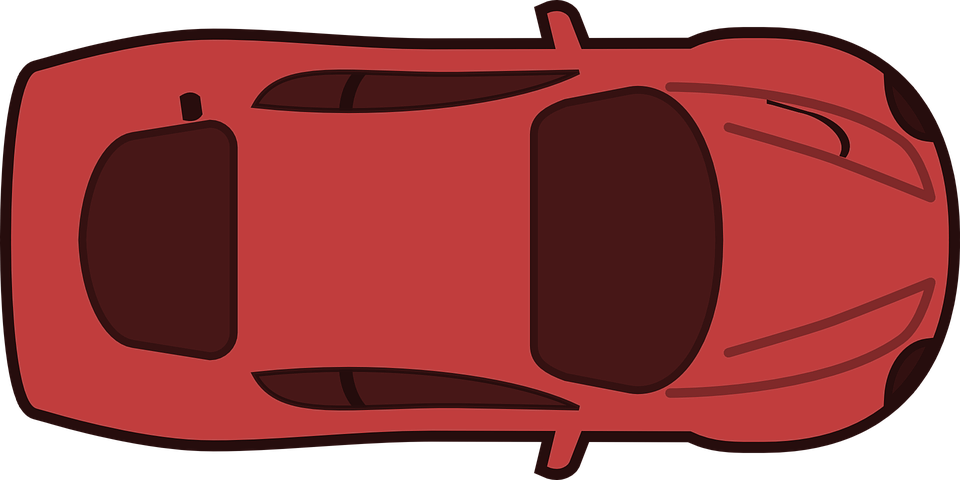
\includegraphics[width=.18\textwidth, angle=0]{figures/ego_car_top_down.png}};
		\draw[->] ([yshift=0.2cm]ego_car.east) -- node[above] {$p_\mathrm{ego}, v_\mathrm{ego}$} ($ (ego_car) + (2.5,0.2)$ );
		% \draw[|-|] ([yshift=-0.2cm]ego_car.east) -- node[below] {$p_{ego}$} (-1,-0.2);
	
		% \node[inner sep=0pt] (target_car_3) at (0,7)
		% {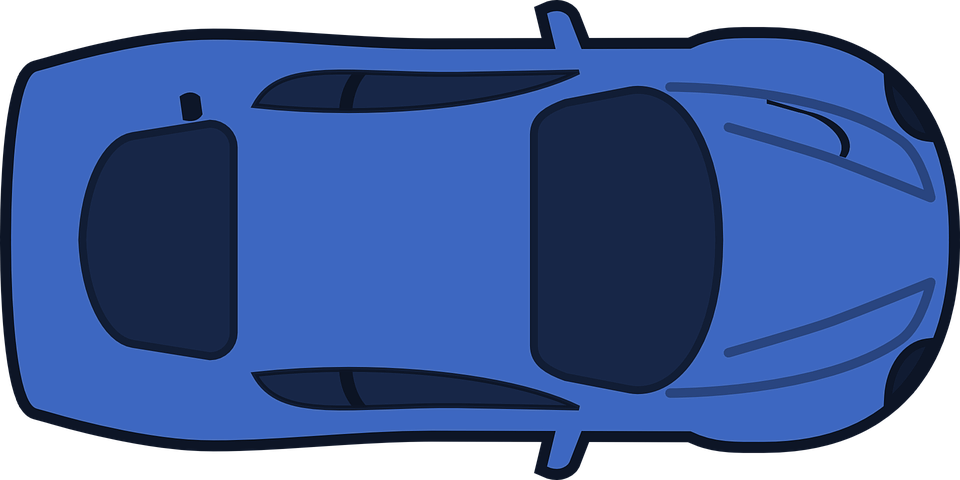
\includegraphics[width=.18\textwidth, angle=-90]{figures/target_car_top_down.png}};
		% \node (tc_text3a) [right=of target_car_3, align=center] {Car $n$};
		% % \node (tc_text3b) [left=of target_car_3, align=center] {Conflict Car};
		% \draw[->] ([xshift=-.3cm]target_car_3.south) -- node[right] {$p_{n} v_{n} \zeta_n$} ($ (target_car_3) + (-.3,-2)$ );
		% \draw[|-|] ([xshift=-0.8cm]target_car_3.south) -- (-.8,1);
		% \node (tc_tti) [below left= 0.9cm and -0.7cm of target_car_3, align=center] {$p_n$  \\ $\tau_{int}$};
	
		\node[inner sep=0pt] (target_car_2) at (0,3.5)
		{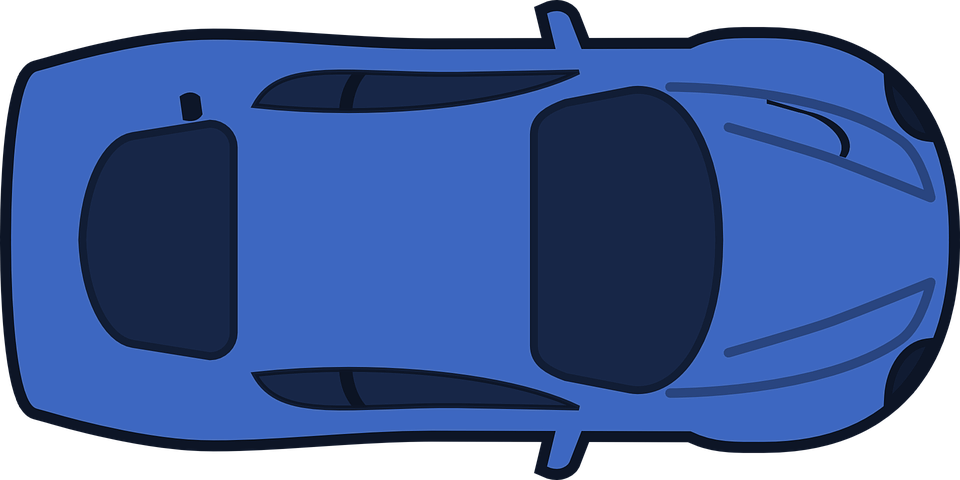
\includegraphics[width=.18\textwidth, angle=-90]{figures/target_car_top_down.png}};
		\node (tc_text2) [right=of target_car_2] {Car $n$};
		\draw[->] ([xshift=-.3cm]target_car_2.south) -- node[right] {$p_{n} v_{n} \zeta_n$} ($ (target_car_2) + (-.3,-2)$ );
		
		\node[inner sep=0pt] (target_car_1) at (0,-1.5)
		{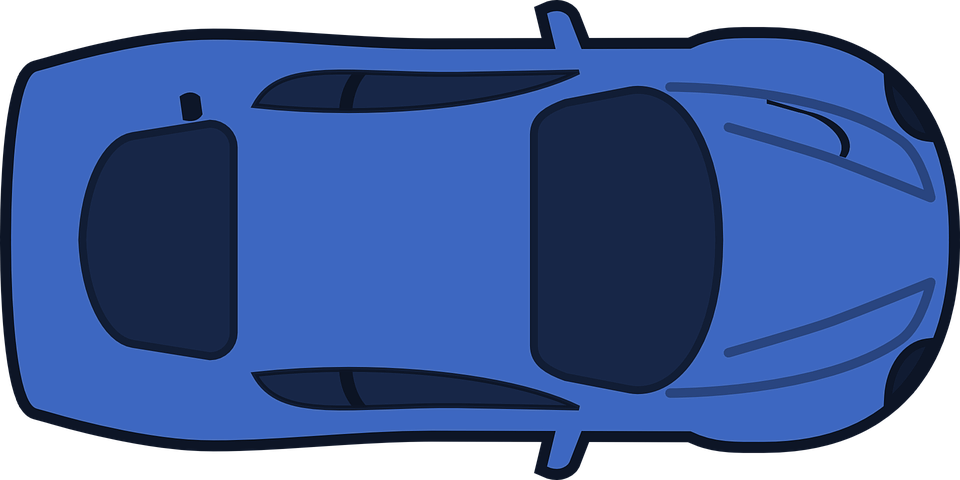
\includegraphics[width=.18\textwidth, angle=-90]{figures/target_car_top_down.png}};
		\node (tc_text1) [right=of target_car_1] {Car 1};
	
	\end{tikzpicture}
	\caption{General description of the states in a simple intersection. The ego vehicle in red is controlled by the agent, while the blue vehicles are the other vehicles crossing the same intersection. Each blue vehicle is described by an index $n$, a position $p_n$, a velocity $v_n$  and hidden intention $\zeta_n$}.
	\label{fig:intersection_scenario}
	\end{figure}

From Section~\ref{sec:background_mdp}, the state space contains all the information necessary about the agent and environment to be able to transition from any given state $s$ to the next state $s'$. In the scenario shown in Figure~\ref{fig:intersection_scenario}, the red car on the horizontal lane represents the ego vehicle controlled by the agent while the blue cars on the vertical lane are the other vehicles which the ego vehicle needs to interact with in order to cross the intersection. 

A simplified description of the state, 
\begin{align}
	s = (p_\mathrm{ego}, v_\mathrm{ego}, \{p_{n}, v_n, \zeta_n\}_{n=1}^N), 
	\label{eq:state}
\end{align}
consists of positions state $p_\mathrm{ego}$ and $p_n$, where subscript \textit{ego} and $n$ denotes the ego vehicle and the index of the surrounding vehicle up to $N$ vehicles. 
% Let's start by defining the information needed. 
Instead of using a Cartesian coordinate system to describe the position $p_\mathrm{ego}$ and $p_n$, relative distance measures are proposed. This way, the state space is generalizable to different intersection designs, e.g., the angle of incidence and the number of crossing points. 
The velocity of ego $v_\mathrm{ego}$ and of all the other traffic participants $v_n$ are also necessary to be able to predict what position they will be in the next state. Finally, the intention of all the other participants $\zeta_n$. As mentioned in Section \ref{sec:intro_intersections}, $\zeta_n$ encapsulates information such as stop sign, traffic light or even inattention in to one variable. 
\paperBelief \ shows a comparison between two fully observable \gls{mdp}s, one with intention and the other one without and the results show that having an intention state reduce number of collisions. 
% \paperLSTM \ used a \gls{lstm} network architecture to implicitly predict $\zeta$. %The states describing ego and other vehicle are spearated. Repeat the states for each other vehicle we observe. 

\subsection{Action space}
\label{sec:pomdp_actionspace}
One limitation of deep Q-learning is the requirement for a discrete action space. In various \gls{ad} studies \cite{bouton2019}, it is common practice to define the action space in terms of different discretized acceleration requests. 
To address the challenge of managing a potentially high-dimensional action space with fine discretization or a coarse action space with large steps between accelerations, Paper A proposes using short-term goals as actions: \{\textit{`take way', `yield', `follow car~$\{1, \dots , N\}$'}\}.

These short-term goals represent high-level objectives, such as driving through an intersection (take way), stopping at the start of an intersection (yield) or drive behind a specific car (follow car~$n$). Each high-level action is translated into a set of parameters that are input into a sliding mode controller in \paperLSTM \ and a \gls{mpc} in \paperMPC, which then generates the appropriate acceleration to control the ego car.

\subsection{Transition model}
\label{sec:pomdp_transistionmodel}
The transition model is initially unknown, and \gls{rl} is employed to implicitly learn this model by taking actions in the environment from different states, recording the resulting rewards, and noting the subsequent state transitions. In this work, the environment is a simulator, and the primary objective for the agent is to learn the transition dynamics of other vehicles, which depend on their intentions $\zeta$. These intentions are modeled as predetermined actions governed by an \gls{idm}. Using the \gls{idm} to guide predetermined actions enhances the dynamics of vehicle interactions, bringing them closer to real-world scenarios. 

\subsubsection{Intelligent Driver Model}
\label{ch:idm}
The \glsfirst{idm} is a widely used car-following model in traffic flow theory and simulation~\cite{idm2000}. It describes how drivers adapt their speed and spacing based on the distance to the vehicle ahead. IDM helps in understanding and predicting traffic dynamics, optimizing traffic flow, and developing \gls{adas} functions. In this thesis the \gls{idm} is used to model the general behavior of surrounding vehicles.
The \gls{idm} models a vehicle $n$'s position $p_n$ and velocity $v_n$ as
\begin{align}
    \dot p_n & = v_n\\
    \dot v_n & = a_{\mathrm{max}}\Big(1-\Big(\frac{v_n}{v^\mathrm{desired}_n}\Big)^\delta-\Big( \frac{d^*(v_n,\Delta v_n)}{d_n}\Big)^2\Big) \label{eq:idm} \\
    & \mathrm{with ~} d^*(v_n, \Delta v_n) = d_0 + v_n T_{\mathrm{gap}} + \frac{v_n \Delta v_n}{2 \sqrt{a_{\mathrm{max}} \alpha_b}} \nonumber
\end{align}
where $v^\mathrm{desired}_n$ is the desired velocity, $d_0$ is the minimum distance between cars, $T_{\mathrm{gap}}$ is the desired time gap to the vehicle in front, $a_\mathrm{max}$ is the maximum vehicle acceleration, $d_n$ is the distance to the vehicle in front, $\Delta v_n = v_n - v_{n-1}$ is the velocity difference between vehicle $n$ and the vehicle directly in front $n-1$, and $\alpha_b$ and $\delta$ are model parameters for comfortable deceleration or acceleration.

The acceleration can be simplified into two terms: an interaction term for when there is a vehicle in front 
\begin{align}
     a^\text{int}_n &=  -a_{max} \Big(\frac{d^*(v_n,\Delta v_n)}{d_n} \Big) ^2  \nonumber \\
     &= -a_{max} \Big(\frac{d_0 + v_n T_{\mathrm{gap}}}{d_n} + \frac{v_n \Delta v_n}{2 \sqrt{a_{\mathrm{max}} \alpha_b} d_n} \Big) ^2
     \label{eq:idm_int}
\end{align}

and free road term, when there is no leading vehicle
\begin{equation}
    a^\text{free}_n= a_\mathrm{max}\Big(1-\Big(\frac{v_n}{v^\mathrm{desired}_n}\Big)^\delta\Big).
    \label{eq:idm_free}
\end{equation}
In this thesis, \gls{idm}'s application ensures realistic simulation of surrounding vehicle behavior, which is crucial for testing and validating the proposed decision-making algorithms for autonomous vehicles.

\subsection{Observation model}
The observation space is closely aligned with the state space $\mathcal{S}$, but it includes some added noise and excludes the intention state $\zeta_n$, because current sensors cannot directly detect the intentions of other drivers.
The observation
\begin{align}
	o = (p_\mathrm{ego}, v_\mathrm{ego}, \{\hat{p}_{n}, \hat{v}_n\}_{n=1}^N), 
	\label{eq:thesis_observation}
\end{align}
encompasses all observable elements of the state, detailed in~\eqref{eq:state}. 
The ego vehicle accurately observes its own states, while it observes noisy measurements of the positions $\hat{p}_{n}$ and velocities $\hat{p}_{n}$ of the surrounding vehicles. These measurements are given by:
\begin{align}
    \label{eq:thesis_noise_pos}
    \hat{p}_{n} = p_{n} + \epsilon_\mathrm{p},\\ 
    \hat{v}_n = v_n + \epsilon_\mathrm{v}
    \label{eq:thsis_noise_vel}
\end{align}
where, $\epsilon_\mathrm{p} \sim \mathcal{N}(0, \sigma^2_p)$ and $\epsilon_\mathrm{v} \sim \mathcal{N}(0, \sigma^2_v)$. 


\subsection{Reward function}
\label{ch:reward_function_def}
The design of the reward function is pivotal as it determines the value associated with each state, ultimately shaping the driving policy of the agent. A well-crafted reward function is instrumental in guiding the agent towards achieving its objectives effectively.
The reward model in this thesis is formulated based on terminal states, including reaching the goal $r^\mathrm{succ}$, collision events $r^\mathrm{fail}$, timeouts $r^\mathrm{t.o.}$, and on non-terminal states $r^\mathrm{comf}$ e.g, every step update the agent has not reached a terminal state. These terminal states play a critical role in defining the success or failure of the agent's driving behavior and are accordingly reflected in the reward structure. One example of a reward function used in this thesis, from \paperMPC, is 
\begin{align}\label{eq:thesis_reward_function}
	r_t = &\begin{cases}
	r^\mathrm{succ} & \text{on success, }\\
	r^\mathrm{fail} & \text{on failure},\\
	r^\mathrm{t.o.} & \text{on timeout, i.e. } \tau \ge \tau_m,\\
	r^\mathrm{comf} & \text{on non-terminating updates},\\
	\end{cases} 
\end{align}
where the reward for reaching the goal is typically assigned a relatively high value, such as $r^\mathrm{succ}=1$, while the reward for colliding is assigned a very low value, such as $r^\mathrm{fail}=-1$. These two rewards establish the maximum and minimum possible rewards for a single simulation run. If the defined reward values are too large, the $Q$-values in \eqref{eq:lossDQN} can become large and cause the gradients to grow and potentially lead to instability~\cite{VanHasseltLearningMagnitude}. Although the absolute values can be chosen arbitrarily, the most important aspect is their relative values to each other. This relative scaling ensures that the agent prioritizes achieving the goal and avoiding collisions appropriately. The other rewards for timeout and non-terminal states are then usually set somewhere between $r^\mathrm{succ}$ and $r^\mathrm{fail}$, such as $r^\mathrm{t.o.}=-0.1$. The reward for non-terminal states $r^\mathrm{comf}$ was utilized differently: \paperLSTM \ used $r^\mathrm{comf}$ to account for comfort by assigning a higher negative reward for high acceleration jerk, while \paperMPC \ added a negative reward was given if the \gls{mpc} predicted a collision.


\section{Simulation environment}
\label{ch:simulation_env}
The simulation environment in this thesis, first introduced in \paperLSTM, places an agent at an intersection tasked with reaching the goal across the intersection while interacting with up to $N$ other cars on the intersecting lane. At the beginning of each episode, up to $N$ vehicles are initialized with initial positions $p_n^0$ distributed along the intersecting lane, starting velocities $v_n^0$ and a deterministic policy that defines their intention $\zeta_n$. 
Each vehicle, including the ego vehicle, adheres to the \gls{idm} (Section~\ref{ch:idm}) aimed at maintaining specific speeds and safe distances, with the maximum acceleration is capped at $5 m/s^2$ to ensure comfort and safety under normal driving conditions.
For example, if a vehicle's intention $\zeta_n$ is yield, it would set the \gls{idm} for the distance to the object in front  $d_n$ to the distance to the start of the intersection, and its velocity $v_{n-1}$ would be set to $0$. Alternatively, a vehicle with a take way intention would follow the IDM only considering the vehicle directly in front of it.

During the simulation, whenever a vehicle in the perpendicular lane crosses the intersection, it is removed from the environment. Subsequently, a new vehicle is spawned at the start of that lane at a random time, with new initial values for position $p_n^0$, velocity $v_n^0$, desired velocity $v^\mathrm{desired}_n$ and intention $\zeta_n$. 
This dynamic spawning process ensures that the traffic scenario continually evolves, presenting varying challenges and interactions for the agent navigating the intersection.
Each episode continues until a terminal state is reached, which can be reaching the goal, collision, or timeout for Paper A-C and goal, collision, safe stop, or deadlock for \paperBelief. Rewards are assigned based on a predefined reward function designed to reinforce desired behaviors. 


\section{Deep Q-learning approach}
To find a driving policy $\pi$ for the \gls{pomdp} detailed in the previous section, both \paperLSTM \ and \paperMPC \ used deep Q-learning, described Chapter~\ref{ch:q-learning}, using a decision-making architecture shown in Figure~\ref{fig:mpc_architecture}. \paperLSTM \ proposed a network architecture with shared weights and \gls{lstm} layer to approximate the Q-function. The shared weight effectively reduces the input space, as the state for each car $n$ can be initially weighted the same as any other car, independent of the order it comes into the neural network. While the \gls{lstm} layer has the role of utilizing the previous states to implicitly estimate a hidden state that could possibly encapsulate the intention of other cars.

\begin{figure}
	\centering
	% \vspace{0.3cm}
	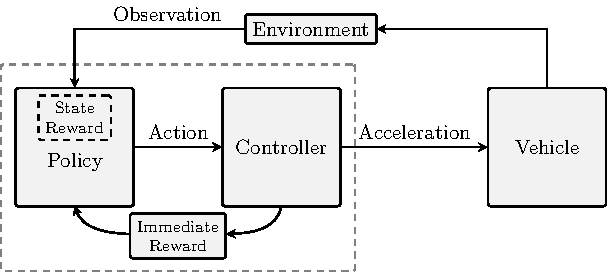
\includegraphics[width=0.8\columnwidth]{YourThesis/papers/mpc/figures/figures-architecture.pdf}
	\caption{Representation of the decision-making architecture. Policy represents the DQN that chooses an action that is sent to a Controller that can either be a sliding mode controller or \gls{mpc}. The Environment represents the simulation environment in which the vehicles operate, but can be replaced by the real world. The State Reward is the reward given by the terminal state ($r^\mathrm{succ},r^\mathrm{fail},r^\mathrm{t.o.}$) from the environment and the Immediate Reward $r^\mathrm{comf}$ is given by the controller.}
	\label{fig:mpc_architecture}
	% \vspace{-0.3cm}
\end{figure}

As mentioned in Chapter~\ref{sec:pomdp_actionspace}, the actions in \paperLSTM \ are controlled by a sliding mode controller while \paperMPC \ uses an \gls{mpc} to generate a velocity profile for a short time horizon. 
The sliding mode controller, which is used interchangeably with the \gls{idm} in this thesis, aims to maintain a minimum distance from a target vehicle by controlling acceleration in a manner similar to \gls{idm}. 

\subsection{Model Predictive Control}
\gls{mpc} is an optimization-based control technique where an Optimal Control Problem (OCP) is repeatedly solved over a receding limited time horizon, starting from the current system state. For every time instance, a mathematical model of the controlled system is used to simulate future states over a finite horizon, while a sequence of control inputs is selected and optimized given an objective cost function. The first element in the sequence of control inputs is then applied to the real system, and a new OCP with an updated state is solved at the next time instance.

\gls{mpc} faces challenges as a mixed integer problem, where calculating the optimal path for all possible actions is computationally intensive. \gls{dqn} on the other hand, only handles discrete actions. While \gls{dqn} cannot guarantee safety, it excels at choosing actions with the highest utility (Q-value). 
The reward function in \gls{dqn} can incorporate the predicted outcome from the \gls{mpc} model, penalizing suboptimal actions. However, if experience shows a better outcome than the model predicts, \gls{dqn} can opt for an action that leads to a better total reward. \paperMPC \ integrates the \gls{mpc} cost as a negative immediate reward, allowing the \gls{dqn} to balance this cost with the high-level goal of reaching the target. This enables the \gls{dqn} to choose actions that are generally beneficial at a high level, even if they may not seem optimal to the \gls{mpc}.

% The reward function in \gls{dqn} can incorporate the predicted outcome from the \gls{mpc} model, penalizing suboptimal actions. However, if experience shows a better outcome than the model predicts, \gls{dqn} can opt for an action that leads to a better total reward compared to strictly following a conservative model.

% \paperMPC \ incorporates the \gls{mpc} cost as a negative immediate reward, the \gls{dqn} can balance the \gls{mpc} cost with the high-level goal of reaching the target, even choosing actions that are generally good at a high level but may not seem optimal to the \gls{mpc}. Instead of specifying which car to drive behind, like the sliding mode controller from \paperLSTM, the action in \paperMPC \ determines which gap between cars the vehicle should drive through. This gap is then translated into constraints that the \gls{mpc} uses to create the velocity profile.

% The agent's objective is to safely track a reference path with target speed, acceleration, and jerk profile, while driving comfortably and avoiding collisions with crossing vehicles at intersections. 
% his is formulated as a finite horizon, constrained optimal control problem:

% \gls{mpc} is good at creating plans within given constraints but faces challenges with mixed integer problems, making the calculation of the optimal path for all possible actions computationally intensive. On the other hand, Q-learning is good at estimating high-return actions based solely on the current state $s$, but requires exploring many suboptimal actions in simulation before converging on a good one. By combining \gls{rl} and \gls{mpc}, the \gls{dqn} can effectively select actions that the \gls{mpc} subsequently utilizes to generate a safe and efficient velocity profile, removing the need to calculate the optimal path for all possible actions.

The agents from \paperLSTM \ and \paperMPC \ are evaluated on two scenarios: a single intersection and a double intersection with two crossing points, both shown in Figure~\ref{fig:example_intersections}. The next section presents the experimental results from \paperLSTM \ and \paperMPC \ for both intersections.

\section{Results from simulation}
\label{sec:results_dqn}
The results from Table~\ref{tab:results_single_double_crossing} show that the proposed \gls{dqn} agent from \paperLSTM \ found a policy that successfully crossed a single intersection $96.1\%$ of the time, with $2.8\%$ resulting in collisions and $1.1\%$ resulting in timeouts. 
When comparing agents trained with and without an \gls{lstm} layer, those with the \gls{lstm} succeeded in 3 out of 4 attempts where those without it would fail.
This demonstrates that deep Q-learning has great potential for creating decision-making agents capable of navigating intersections. OA key contribution of this thesis is the proposal of network architectures specifically designed for this problem. In \paperLSTM, an architecture employing shared weights is introduced, and the results shown in Figure~\ref{fig:results_shared} reveal that utilizing a network with shared weights for processing information about observed vehicles notably enhances convergence speed. The combination of shared weights with other improvements, such as dropout and experience replay, is crucial for achieving these performance gains.


\begin{figure}[!ht]
	\centering
	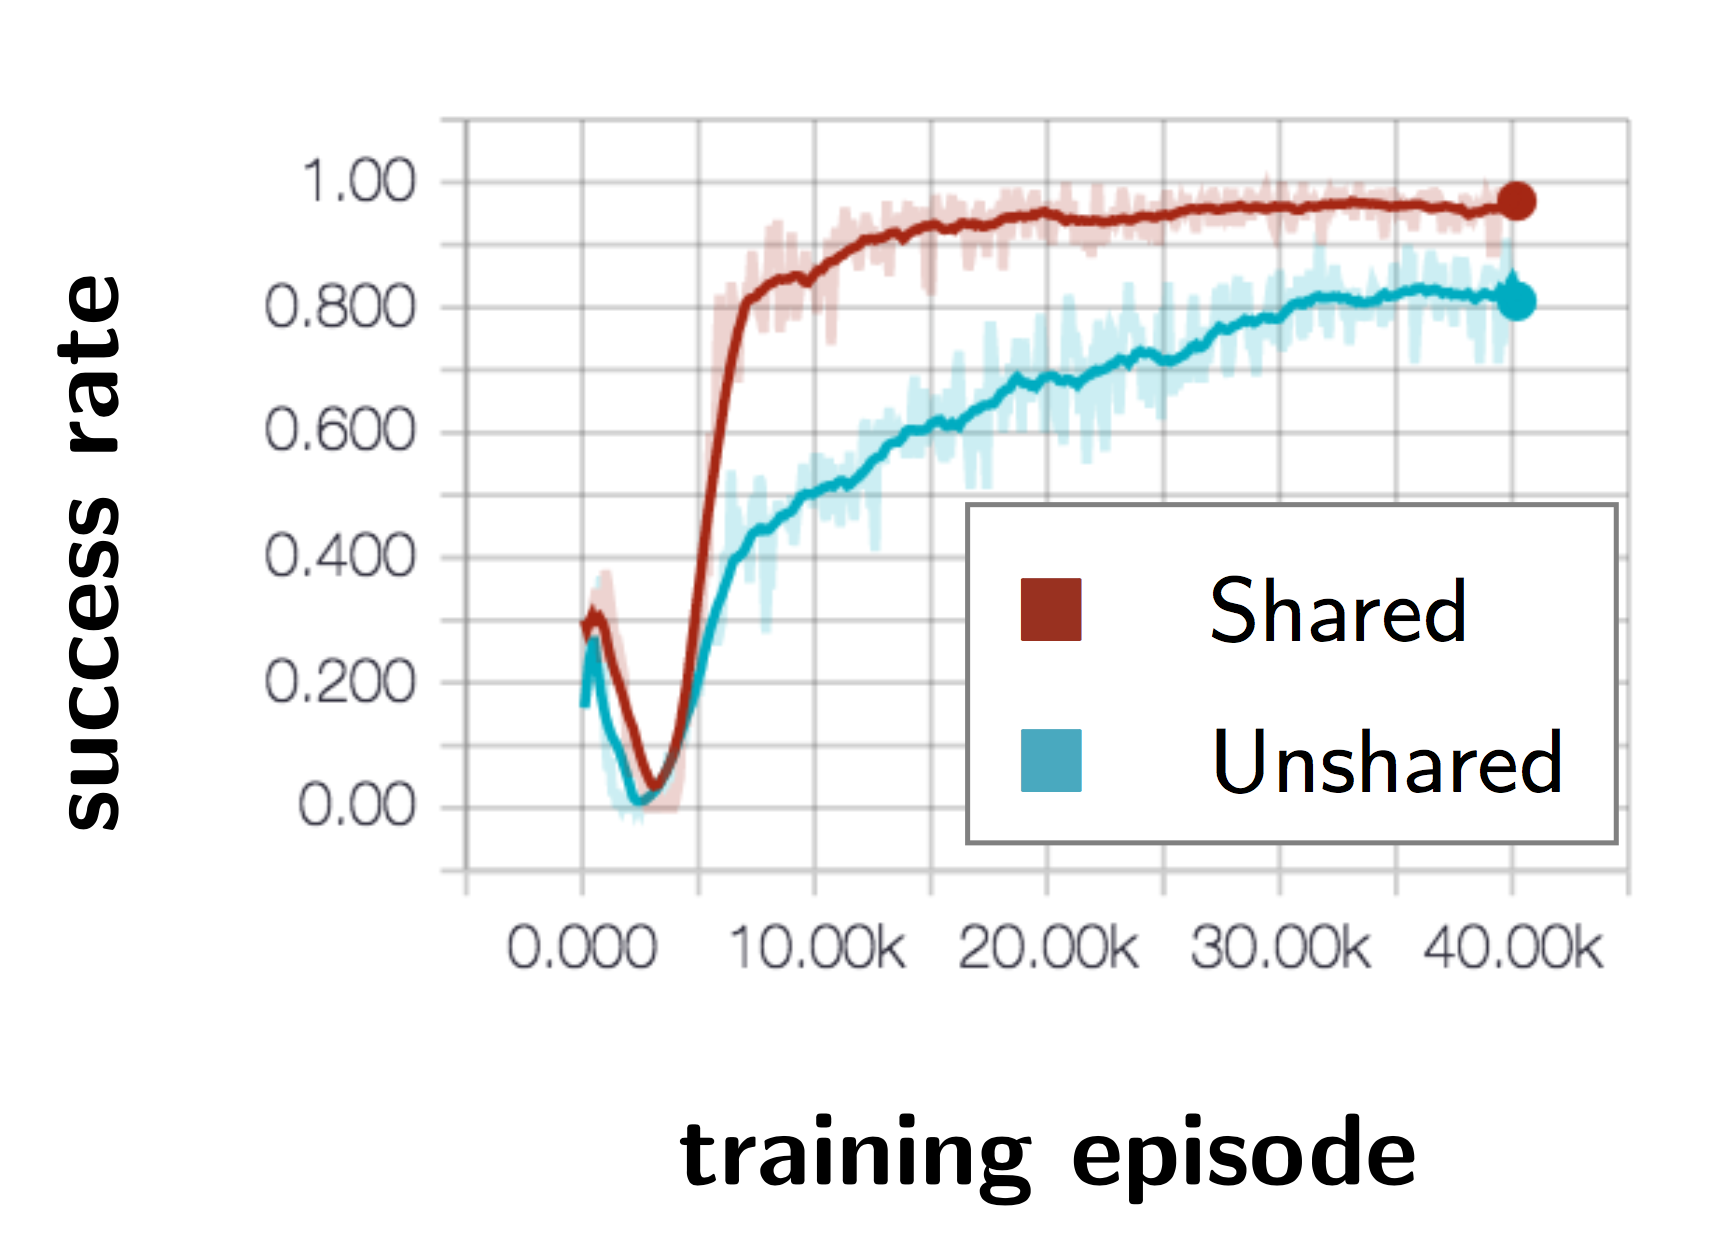
\includegraphics[width=0.7\columnwidth]{YourThesis/papers/lstm/figures/results_shared.png}
	\caption{The figure shows that the success rate for a network with shared weights (brown line) converge faster than the fully connected network structure which do not share weights (turquoise line).}
	\label{fig:results_shared}
\end{figure}

As mentioned in Section~\ref{sec:pomdp_actionspace}, the controller from \paperLSTM \ could only consider one car at a time e.g., follow car $n$. 
If the agent needs to achieve a velocity between two discrete actions, it can do so by switching between them in a manner similar to pulse-width modulation. However, this placed a heavy burden on the \gls{dqn} compensate by frequently switching actions. 
In contrast, in \paperMPC, the \gls{mpc} showed significant improvement in handling more complex intersections.
For instance, in the double intersection, the \gls{mpc} agent succeeded $95.2\%$ of the time with a collision rate of $3.6\%$, compared to the sliding mode controller, which only succeeded $90.9\%$ of the time with a collision rate of $8.3\%$. 

% \begin{figure}[!ht]
% 	\centering
% 	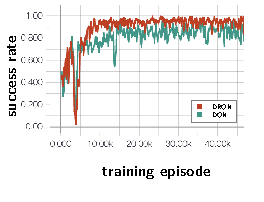
\includegraphics[width=0.7\columnwidth]{figures/figures-recurrent.pdf}
% 	\vspace{-0.5cm}
% 	\caption{Graphs presenting the performance of a DRQN (red) compared to a DQN with a single observation (green), running on scenarios with cars that have different behaviors. When compared a DRQN succeeds in 3 out of 4 attempts, where a DQN fails.}
% 	\label{fig:results_recurremt}
% \end{figure}

% \begin{figure}[t!]
	% \mbox{\parbox{\textwidth}{
% 	\centering
% 	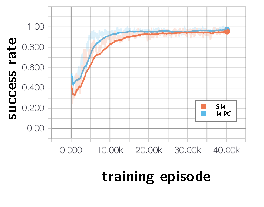
\includegraphics[width=\columnwidth]{YourThesis/papers/mpc/figures/figures-successrate.pdf}
% }}
% 	\caption{Average MPC and SM success rate for a single corssing after evaluating the policy 300 episodes.}
% 	\label{fig:result1}
% \end{figure}

% \begin{figure}[t!]
% 	\centering
% 	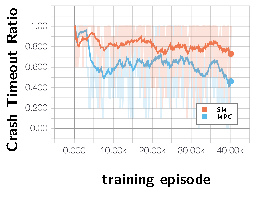
\includegraphics[width=\columnwidth]{YourThesis/papers/mpc/figures/figures-crashratio.pdf}
% 	\vspace{-4em}
% 	\caption{Average MPC and SM crash to timeout ratio for a single crossing after evaluating the policy in 300 episodes. A CTR of $0$ means that all failures are timeouts, while a CTR of $1$ means that all failures are collisions.}
% 	\label{fig:result2}
% \end{figure}

\begin{table}[h]
	\mbox{\parbox{\textwidth}{
	\centering
	\begin{tabular}{ |p{2,6cm}||p{1,2cm}|p{1,2cm}|p{1,2cm}|p{1,2cm}|}
	\hline
	Controller &\multicolumn{2}{|c|}{Success Rate}&\multicolumn{2}{|c|}{Collision Rate}\\
	\hline
	 & Single & Double & Single & Double\\
	\hline
	SM (\paperLSTM) & $96.1\%$ & $90.9\%$ & $2.8\%$ & $8.3\%$\\
	MPC (\paperMPC) & $97.3\%$ & $95.2\%$ & $1.2\%$ & $3.6\%$\\
	\hline
	\end{tabular}
	}}
	\caption{Average success rates and collision rates for a fully trained \gls{dqn} agent driving through a single and double intersections. If the agent failed to reach the goal or collide within a given time, the terminal state was classified as a timeout.}% across single and double crossings.}   
\label{tab:results_single_double_crossing}
\end{table}


\section{Discussion}
% \section{The intersection problem}
\begin{figure}
	\mbox{\parbox{\textwidth}{
		\centering
		\begin{tikzpicture}
			\def\xstart{-7};

			\coordinate (p) at (3,0);
			\foreach \n/\w/\c in {z0/2/green,z1/2/red,z2/2.5/orange,z3/3.5/blue}{
				\node[rectangle,
				draw=none,
				anchor=east,
				text = black,
				fill = \c!60,
				minimum width = \w cm, 
				minimum height = 2cm] 
				(n) at (p) {\Huge \n};
				
				\coordinate (p) at (n.west);
			}

			% Crossing
			\draw[line width=0.5mm] (\xstart, 1) -- (-1, 1) -- (-1, 5);
			\draw[line width=0.5mm] (\xstart, -1) -- (-1, -1) -- (-1, -2);
			\draw[line width=0.5mm] (1, 5) -- (1, 1) -- (3, 1);
			\draw[line width=0.5mm] (1, -2) -- (1, -1) -- (3, -1);
			
			% cars
			\node[inner sep=0pt] (ego_car) at (-7,0)
			{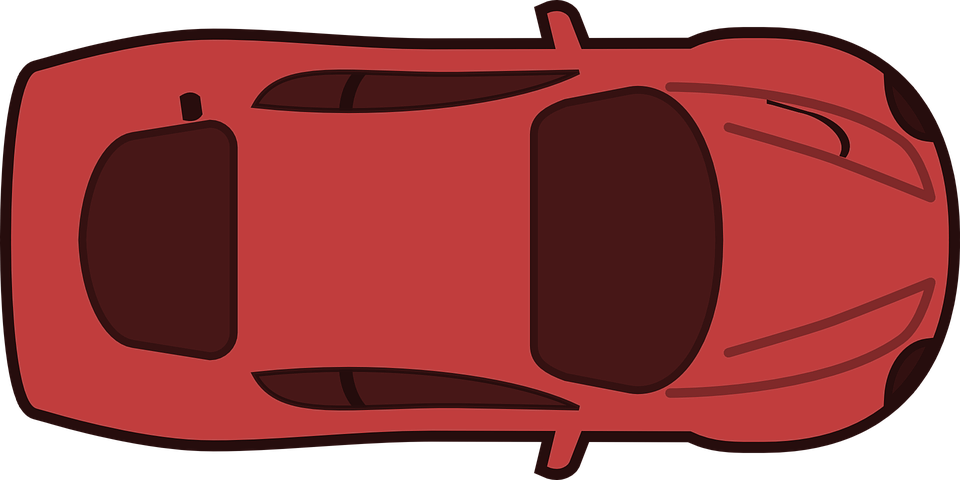
\includegraphics[width=.18\textwidth, angle=0]{figures/ego_car_top_down.png}};
			\node[inner sep=0pt] (target_car) at (0,4)
			{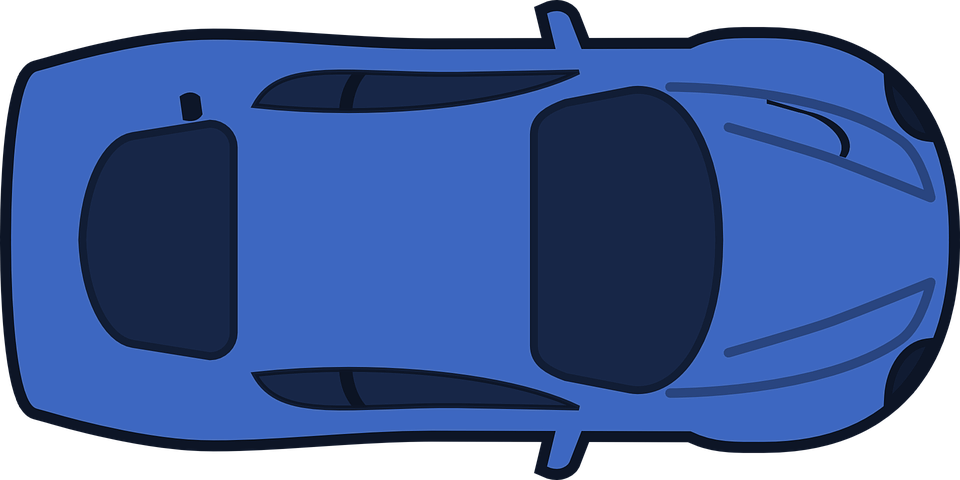
\includegraphics[width=.18\textwidth, angle=-90]{figures/target_car_top_down.png}};

	\end{tikzpicture}
	}}
	\caption{Intersection scenario divided into zones describing what is required of the decision maker in different zones}
	\label{fig:zones}
\end{figure}

Observing the behavior of a fully trained agent from \paperLSTM \ and \paperMPC \ provides the insight that the path of the ego vehicle can be segmented into four zones, illustrated in Figure~\ref{fig:zones}. Starting from the right, Zone 0 represents the \textit{safe zone}, where the ego vehicle is out of danger and can resume nominal driving. Zone 1 is the \textit{conflict zone}, where a collision with another vehicle is possible. Zone 2, the \textit{critical decision zone}, is the final opportunity for the vehicle to either stop or proceed through the intersection. The size of zone 2 is determined by the minimum distance required for the vehicle to come to a complete stop before entering the conflict zone, ensuring sufficient time for safe decision-making. Lastly, Zone 3, the \textit{information gathering zone}, is situated furthest from the intersection. Here, the agent can observe how other vehicles behave over time to estimate their intentions.

The goal is to reach Zone 0. To achieve this, the agent aims to minimize the time spent in Zone 1 if there is a chance of intersection with another car. Our actions are formulated as short-term goals, designed for comfortable use with lower acceleration rates. The size of Zone 2 depends on the vehicle's current speed, which is influenced by its behavior in Zone 3.

Now, two conflicting strategies emerge: to minimize time in Zone 1, the agent desires a high speed entering the intersection. However, it also seeks a low speed to reduce the size of Zone 2 and the critical decision period. If the intentions of other vehicles are known, the stochasticity in Zone 1 would be eliminated, transforming the problem into a scheduling task aimed at creating a velocity profile that minimizes the time required to cross. However, since the intentions of other vehicles are inherently stochastic, the next chapter offers a promising approach by accounting for this uncertainty and optimizing decision-making in dynamic traffic scenarios.


